\newpage

\section{Primera Parte: Estimación de RTT}
En esta primera parte del trabajo, el objetivo es realizar mediciones de
\emph{round-trip time} tanto teóricas como empíricas y razonar alrededor de
los resultados.

\subsection{Caracterización de los experimentos}

Elegimos tres universidades en distintas partes del mundo (Cambridge
University, Inglaterra; Stanford University, Estados Unidos; Moscow State
University, Rusia) y, tomando la dirección IP del dominio principal de cada
una, realizamos las siguientes mediciones:
\begin{enumerate}
    \item \textbf{Cálculo del RTT teórico.} Para esto, primero definimos la
        ubicación geográfica de la dirección haciendo uso de un servicio de
        geolocalización. Con ella, calculamos la distancia lineal desde ese
        punto hasta el que sería el origen de nuestras mediciones. Tomando un
        tiempo de propagación de la señal de $2 \times 10^5$ km/s, calculamos
        el tiempo que tardaría la ida de un paquete hasta el servidor destino
        y la llegada de una respuesta o reconocimiento inmediato.
    \item \textbf{Medición de RTT teórico teniendo en cuenta el camino
        recorrido por los paquetes.} Similar al cálculo teórico anterior, esta
        vez teniendo en cuenta las ubicaciones geográficas de cada uno de los
        routers intermedios.
    \item \textbf{Medición de RTT mediante una herramienta propia.} Utilizando
        una herramienta de \emph{traceroute} desarrollada por nosotros usando
        la biblioteca Scapy, calculamos el RTT empírico a la dirección
        destino.
    \item \textbf{Medición de RTT mediante una herramienta del sistema
        operativo.} Idéntico al caso anterior pero esta vez usando el
        \emph{traceroute} disponible en una distribución de GNU/Linux.
\end{enumerate}

Previamente a las mediciones, se esperaba que el RTT teórico lineal fuera, en
general, muy menor a los obtenidos empíricamente, puesto que este, además de
dejar de lado retardos ocasionados por los routers en distintas horas del día,
asumía la existencia de un medio de comunicación (fibra óptica) cubriendo la
menor distancia entre el origen y el destino de la medición. Dado que el RTT
teórico del camino no asume esto último, se esperaba que este, si bien fuera
menor a los valores empíricos, se ajustara más a estos.

Por otro lado, se esperaba ver que los valores de RTT empíricos arrojados por
ambas herramientas de \emph{traceroute} fueran cercanos, ya que las mediciones
se realizarían en condiciones similares y los métodos para realizar los
cálculos serían parecidos.

Asimismo, como realizaríamos mediciones para distintos momentos del día, se
esperaba ver diferencias en los RTT según el horario, aunque no se suponía
ningún patrón en particular.

\subsection{Resultados de los experimentos}

\begin{figure}[h!]
    \centering
    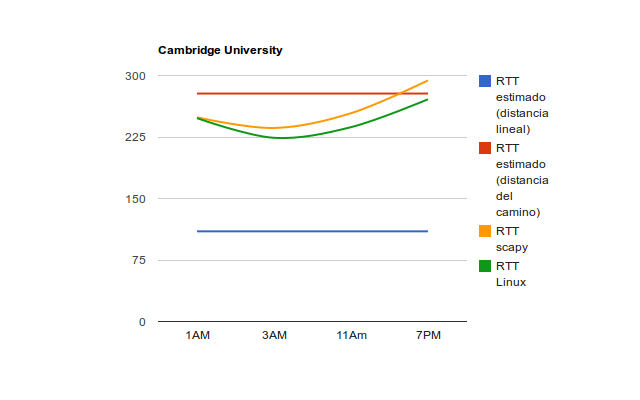
\includegraphics[width=400pt]{cambridge.png}
    \caption{Cambridge University}
    \label{fig:cambridge:count}
\end{figure}

\begin{figure}[h!]
    \centering
    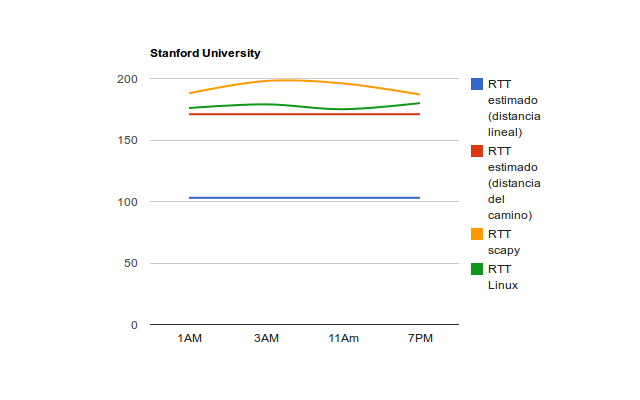
\includegraphics[width=400pt]{stanford.png}
    \caption{Stanford University}
    \label{fig:stanford:count}
\end{figure}

\begin{figure}[h!]
    \centering
    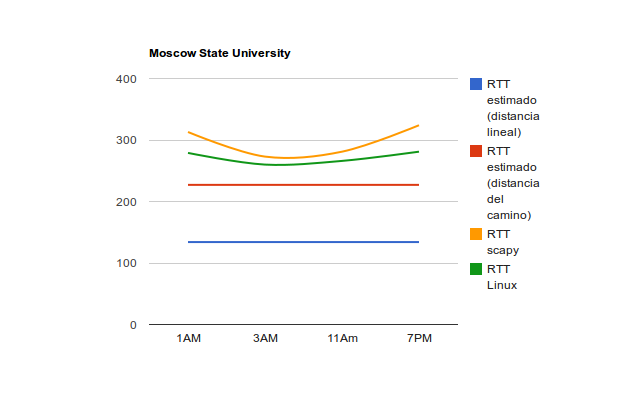
\includegraphics[width=400pt]{msu.png}
    \caption{Moscow State University}
    \label{fig:msu:count}
\end{figure}

\begin{figure}[h!]
    \centering
    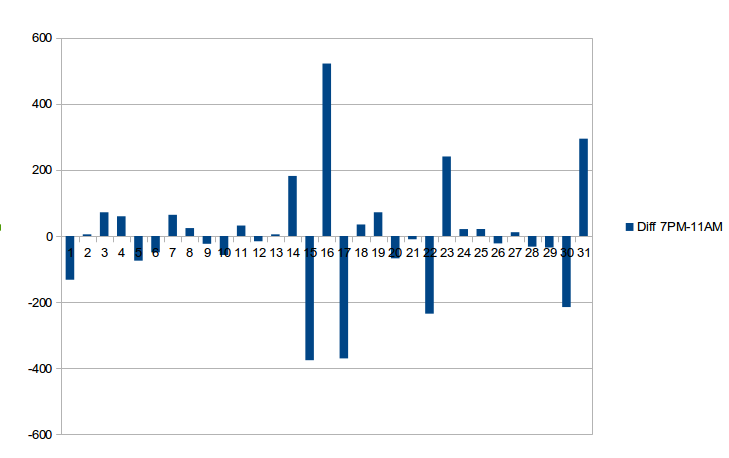
\includegraphics[width=400pt]{cambridge-diff-7PM-11AM.png}
    \caption{Diferencias entre RTTs para los enlaces de la ruta a Cambridge
    University}
    \label{fig:cambridge:diff}
\end{figure}

Las figuras \ref{fig:cambridge:count}, \ref{fig:stanford:count} y
\ref{fig:msu:count} muestran las mediciones para la Cambridge University
(Inglaterra), Stanford University (Estados Unidos) y la Moscow State
University (Rusia) respectivamente.

En cada uno de estos gráficos puede verse una curva interpolada que muestra,
para distintos horarios del día, los \emph{round-trip times} consignados en
milisegundos, medidos según los métodos antes descriptos.

La figura \ref{fig:cambridge:diff} muestra la diferencia entre los horarios de
las 7PM y las 11AM de los RTTs para los enlaces de la ruta hasta el servidor
de la Cambridge University.

\subsection{Análisis de los resultados}
De los gráficos resultantes de los experimentos, pueden observarse varias
cosas que discutiremos a continuación.

En primer lugar, observamos que, efectivamente, el RTT teórico que considera
el camino se acerca más a los valores empíricos que el RTT teórico lineal. La
justificación es, como se dijo antes, que este RTT no asume que el origen y
destino de los experimentos están conectados mediante un medio (fibra óptica)
que los une cubriendo la menor distancia, sino que tiene en cuenta las
desviaciones por los routers intermedios.

No obstante, cabe mencionar que, a diferencia de lo que se esperaba, este RTT
dio, para el caso de la Cambridge University, valores mayores a los empíricos.
Creemos que esto puede deberse a un error en la herramienta de geolocalización
utilizada (hay un desvío de unos 1000 km en uno de los últimos \emph{hops}).
También puede estar sucediendo que ese hop, que tiene una IP de Escocia, en
realidad sea un servidor ubicado en Inglaterra pero que por alguna razón tiene
una IP del primer país. Algo similar ocurre con uno de los primeros hops, que
tiene una IP de Estados Unidos pero el RTT medido a ese host es de 28ms, un
valor más acorde a un host nacional.

Por otro lado, se observa que, en los horarios de la madrugada, hora local, el
RTT disminuye en las dos rutas hacia Europa. Entendemos que esto se debe a que
en esos horarios el tráfico es menor tanto en el origen como en el destino.
Esto no se da de la misma forma en la ruta hacia Estados Unidos, ya que, al
ser en la costa oeste 4 hs menos que en Buenos Aires, a esa hora todavía se
registra un tráfico alto.

Además, vimos que los resultados de las dos herramientas son bastante
similares. Probablemente el hecho de que la implementación de
\emph{traceroute} del sistema operativo haga 3 intentos por hop sea la razón
por la cual su curva es más suave.

En cuanto a los tiempos de encolado, si bien, como ya se dijo, pudimos
observar diferencias en los RTTs a los servidores de las universidades para
diferentes momentos del día, lo cual atribuimos a los cambios en el tráfico en
cada lugar, nos fue imposible realizar análisis más detallados en cuanto a los
enlaces particulares de cada ruta. Se daban muchos
casos en los cuales la variabilidad de los valores era tan grande que no nos
permitía sacar ninguna conclusión.

Definimos el RTT de un enlace entre los hosts $h_i$ y $h_{i+1}$ como el RTT de
$h_{i+1}$ al origen menos el RTT de $h_i$ al origen, y luego observamos el RTT
de los enlaces para distintos horarios del día. Por ejemplo, el gráfico
\ref{fig:cambridge:diff} muestra las diferencias entre RTTs para los enlaces
en la ruta al servidor de la Cambridge University entre el horario de las 7PM
y las 11AM. En este gráfico puede verse cómo los enlaces 15, 16 y 17, todos
entre nodos ubicados en Estados Unidos, muestran una diferencia muy grande.
Estas diferencias no nos permitieron arribar a conclusiones relacionadas con
el tráfico en esos horarios determinados, en las diferentes zonas geográficas,
y su influencia en los tiempos de encolamiento en los nodos.
